\documentclass[a4paper, 12pt]{article}

\usepackage{hyperref}
\usepackage[warn]{mathtext}
\usepackage[utf8]{inputenc}
\usepackage[T2A]{fontenc}
\usepackage[english,russian]{babel}
\usepackage{multirow}
\usepackage{float}
\restylefloat{table}
\usepackage{amsmath,amsfonts,amssymb,amsthm,mathtools}
\usepackage{indentfirst}
\DeclareSymbolFont{T2Aletters}{T2A}{cmr}{m}{it}
\usepackage{ gensymb }
\mathtoolsset{showonlyrefs=true}
\usepackage{euscript}
\usepackage{mathrsfs}
\usepackage[left=2cm,right=2cm,top=2cm,bottom=2cm]{geometry}
\usepackage{graphicx}
\usepackage{wrapfig}
\usepackage[rgb]{xcolor}
\hypersetup{
colorlinks=true,
urlcolor=blue
}
\usepackage{siunitx}
\usepackage{tikz}

\unitlength=1mm

\title{ВПВ}
\author{Гисич Арсений Б03-102}
\date{2023}

\begin{document}

	\begin{center}
		{\large МОСКОВСКИЙ ФИЗИКО-ТЕХНИЧЕСКИЙ ИНСТИТУТ (НАЦИОНАЛЬНЫЙ ИССЛЕДОВАТЕЛЬСКИЙ УНИВЕРСИТЕТ)}
	\end{center}
	\vspace{5 cm}
	{\Large
		\begin{center}
			{\bf Вопрос по выбору}\\[0.2 cm]
			<<Духи>> Роуланда
		\end{center}
	}
	\vspace{4 cm}
	\begin{flushright}
		{\Large Автор: \\
			\vspace{0.2 cm}
			Гисич Арсений \\
			\vspace{0.2 cm}
			Б03-102 \\}
	\end{flushright}
	\vspace{8 cm}
	\begin{center}
		Долгопрудный\\[0.1 cm]
		2023
	\end{center}
\thispagestyle{empty}

\begin{abstract}
У реальных дифракционных решёток могут быть разнообразные ошибки в расположении штрихов, проявляющиеся в нарушении их периодичности. Каждый винт делительной машины имеет периодическую ошибку нарезки, и она приводит к периодическим ошибкам в расположении штрихов. Это сказывается в появлении около каждой спектральной линии ложных линий, симметрично расположенных относительно основных и получивших название <<духов Роуланда>>.
\end{abstract}

Для волны длины $\lambda$, падающей под углом $i$ на дифракционную решётку, направления $\theta$ на дифракционные максимумы выражаются формулой 
\begin{equation} \label{eq:dif_grating}
d (\sin{i} + \sin{\theta}) = N \lambda,
\end{equation}
где $d$ --- период решётки, $N$ --- порядок максимума.

Если $m$ --- период винта делительной машины, то расстояние от края решётки до n-го штриха выражается как
\begin{equation} \label{eq:err_pos}
y = d_0 n + d_1 \sin{e_1 n} + d_2 \sin{e_2 n} + \ldots,
\end{equation}
где $e_k = 2\pi/m_k$ и $d_k$ --- максимальное отклонение любого штриха от корректного положения вследствие ошибки $e_k$.

Введём обозначения:
\begin{equation} \label{eq:new_var}
\begin{aligned}[t]
\xi &= \sin{\alpha} + \sin{\alpha'}, \\
\mu &= \sin{i} + \sin{\theta} = \frac{2 \pi N}{k d_0},
\end{aligned}
\end{equation}
где $\alpha$ и $\alpha'$ --- направление падающего и дифрагировавшего луча относительно оси $X$. Тогда колебание напряжённости электрического поля в плоскости экрана пропорционально
\begin{equation} \label{eq:int}
\sum{\int_{y'}^{y''} e^{-i k(\xi x + \mu y)} ds} = \sum{e^{-i k \mu y'}} \int_{0}^{y'' - y'} e^{-i k(\xi x + \mu_y)} ds.
\end{equation}
Для упрощения можно принять $y'' - y' = d_0$, тогда из под знака интеграла можно вынести сумму
\begin{equation} \label{eq:err_sum}
\sum{e^{-i k \mu(d_0 n + d_1 \sin{e_1 n} + d_2 \sin{e_2 n} + \ldots)}}.
\end{equation}

Пусть $J_n$ --- функция Бесселя. Тогда 
\begin{equation} \label{eq:bess}
\begin{aligned}
\cos{(u \sin{\varphi})} &= J_0(u) + &2[J_2(u) \cos^2{\varphi} + J_4(u) \cos^4{\varphi} + \ldots] \\
\sin{(u \sin{\varphi})} &= &2[J_1(u) \sin{\varphi} + J_3(u) \sin^3{(\varphi)} + \ldots]
\end{aligned}
\end{equation}

Также $e^{-i u \sin{\varphi}} = \cos{(u \sin{\varphi})} - i \sin{(u \sin{\varphi})}$. Тогда сумма преобразуется как
\begin{equation} \label{eq:sum_bess}
\sum {}
	\begin{cases}
	\quad e^{-ik\mu d_0 n} \\
	\times [J_0(k\mu d_1) + 2(-i J_1(k \mu d_1) \sin{e_1 n} + J_2(k \mu d_1) \cos{2 e_1 n} - \ldots)] \\
	\times [J_0(k\mu d_2) + 2(-i J_1(k \mu d_2) \sin{e_2 n} + J_2(k \mu d_2) \cos{2 e_2 n} - \ldots)] \\
	\times [J_0(k \mu d_3) + \ldots] \\
	\times [\ldots]
	\end{cases}
\end{equation}

В простейшем случае все $d_k$ равны нулю, кроме $d_0$ и $d_1$. Используя формулу
\begin{equation} \label{eq:progr_sum}
\sum_0^{n - 1}{e^{-i p n}} = e^{-i \frac{n - 1}{2}p}{\frac{\sin{\frac{p n}{2}}}{\sin{\frac{p}{2}}}}.
\end{equation}
находим выражение для интенсивности
\begin{equation}\label{eq:intens}
\left\{ J_0(k \mu d_1) \frac{\sin{n\frac{k \mu d_0}{2}}}{\sin{\frac{k \mu d_0}{2}}}\right\}^2 + J_1^2(k \mu d_1) \left\{ \left\{ \frac{\sin{n \frac{k \mu d_0 + e_1}{2}}}{\sin{\frac{k \mu d_0 + e_1}{2}}} \right\}^2 + \left\{ \frac{\sin{n \frac{k \mu d_0 - e_1}{2}}}{\sin{\frac{k \mu d_0 - e_1}{2}}} \right\}^2 \right\} + \ldots
\end{equation}
Здесь $u = k \mu_p d_1 = (2 \pi[N + (p/m)] d_1 / d_0)$, откуда можно получить выражение для длин волн, соответствующих <<духам>>:
\begin{equation} \label{eq:new_wlen}
\lambda_p = \lambda \left(1 \pm \frac{p}{N m}\right).
\end{equation}

Так как $n$ --- велико, это выражение даёт очень узкие спектральные линии, которые не накладываются и, как следствие, могут быть различимы. Соответствующие позиции спектральных линий и их <<духов>> представлены в таб.~\ref{tab:ghosts_pos}. На рис.~\ref{fig:intens} изображена зависимость интенсивностей <<призраков>> различных порядков от соотношения $d_1/d_0$.

\begin{table}[h!]
\renewcommand{\arraystretch}{1.5}
\begin{center}
\begin{tabular}{|c|c|c|}
\hline 
Расположение & Интенсивность & Обозначение \\ 
\hline 
$\mu = \frac{2 \pi N}{k d_0} $ & $J_0^2(k \mu d_1)$ & первоначальная линия \\ 
\hline 
$\mu_1 = \mu \pm \frac{e_1}{k d_0}$ & $J_1^2(k \mu_1 d_1)$ & <<призраки>> 1-го порядка \\ 
\hline 
$\mu_2 = \mu \pm \frac{2 e_1}{k d_0}$ & $J_2^2(k \mu_2 d_1)$ & <<призраки>> 2-го порядка \\ 
\hline 
$\mu_3 = \mu \pm \frac{3 e_1}{k d_0}$ & $J_3^2(k \mu_3 d_1)$ & <<призраки>> 3-го порядка \\ 
\hline 
\end{tabular}
\end{center}
\caption{Расположение соответствующих спектральных линий и их <<духов>>}
\label{tab:ghosts_pos}
\end{table}

\begin{figure}[h!]
\begin{center}
    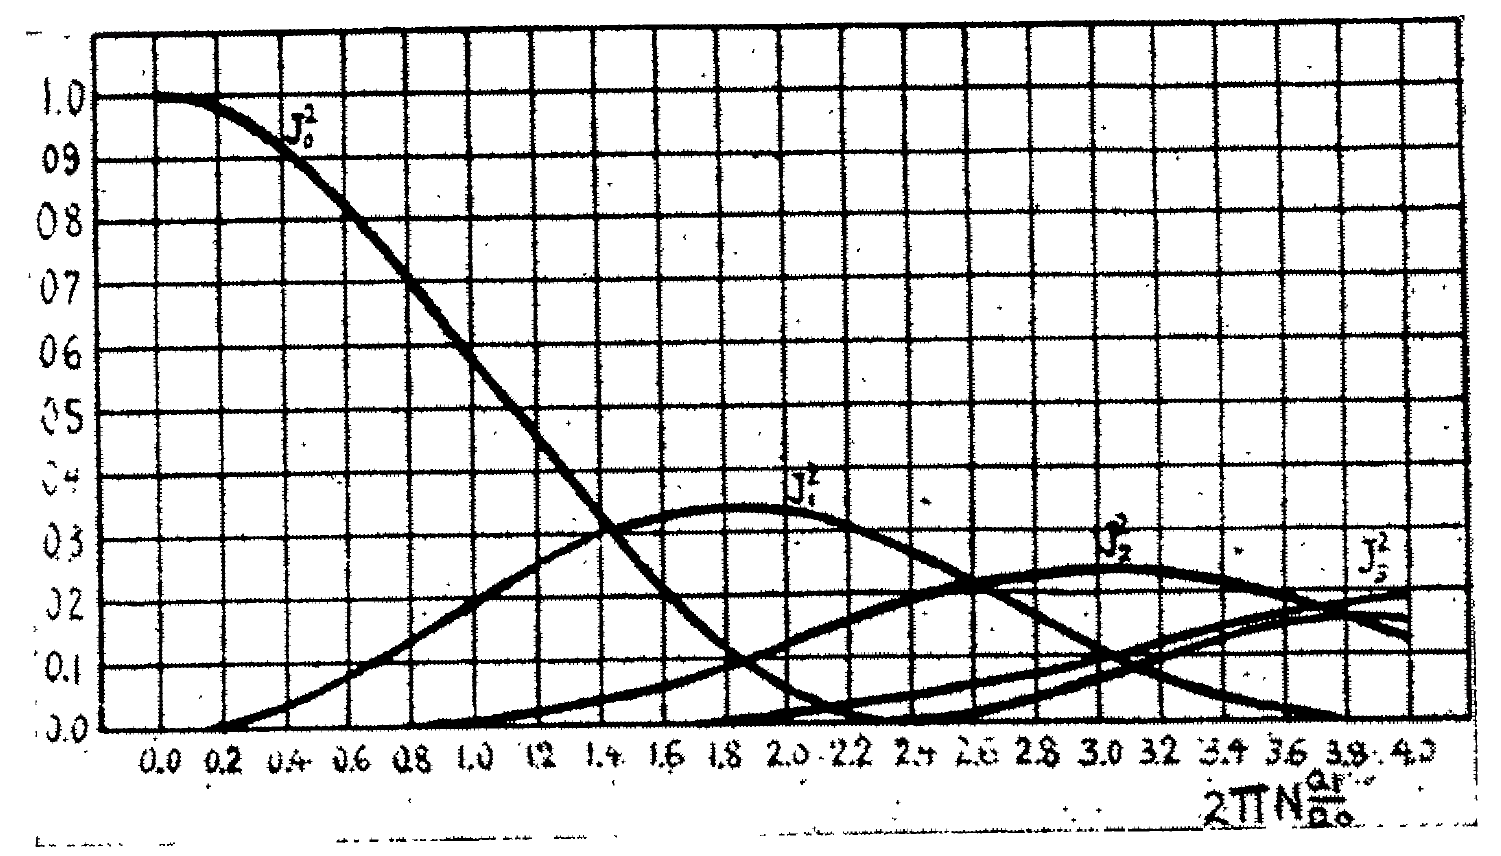
\includegraphics[width=0.8\textwidth]{intens.png}
\end{center}
\caption{График зависимости интенсивности $J_n$ от отношения $d_1/d_0$}
\label{fig:intens}
\end{figure}

\begin{figure}[h!]
\begin{center}
    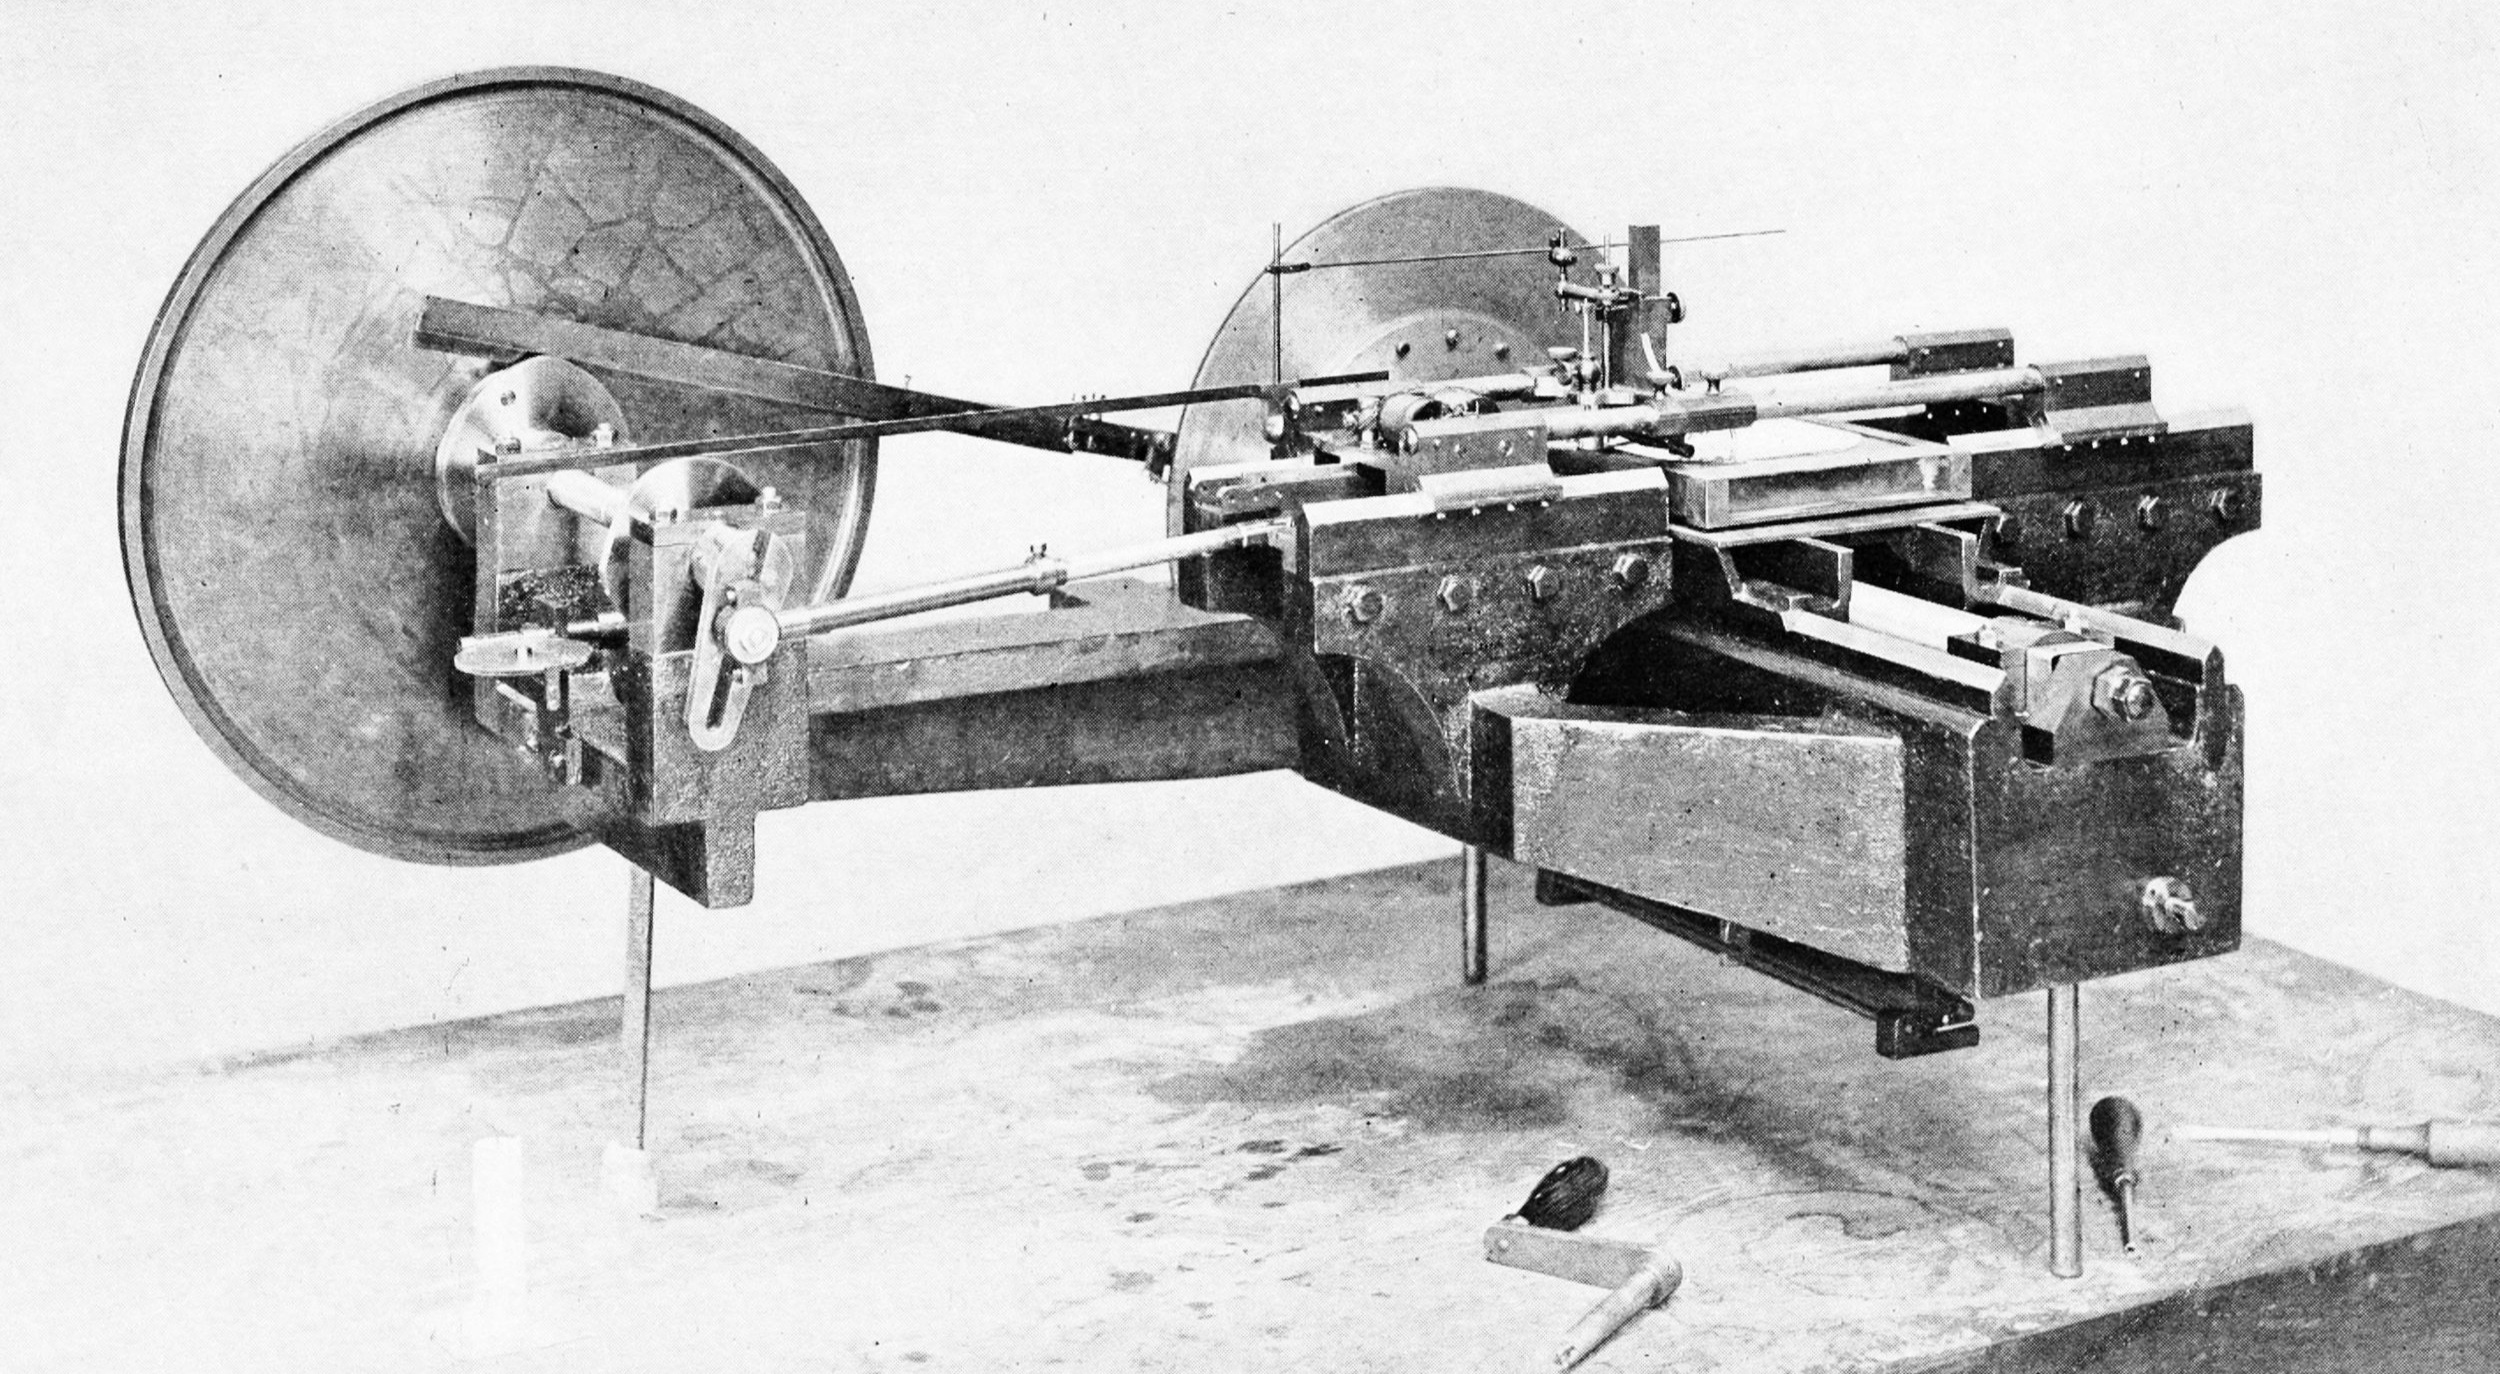
\includegraphics[width=0.8\textwidth]{machine.jpg}
\end{center}
\caption{Делительная машина Роуланда}
\label{fig:machine}
\end{figure}

Общий вид делительной машины Роуланда представлен на рис.~\ref{fig:machine}. Управляющий механизм делительной машины оснащён компенсационным цилиндром \textit{C} (рис.~\ref{fig:engine}), который удерживает длинный конец рычага \textit{L}. Короткий конец рычага несёт наконечник \textit{B} шнека \textit{W}, который вращает шнековое колесо \textit{A}. В начале цилиндр был настроен так, чтобы убрать любые ошибки вращения. Затем на компенсатор добавлялись различные ошибки. Результаты экспериментов, проведённых в Ryerson Physical Laboratory, представлены далее.

\begin{figure}[h!]
\begin{center}
    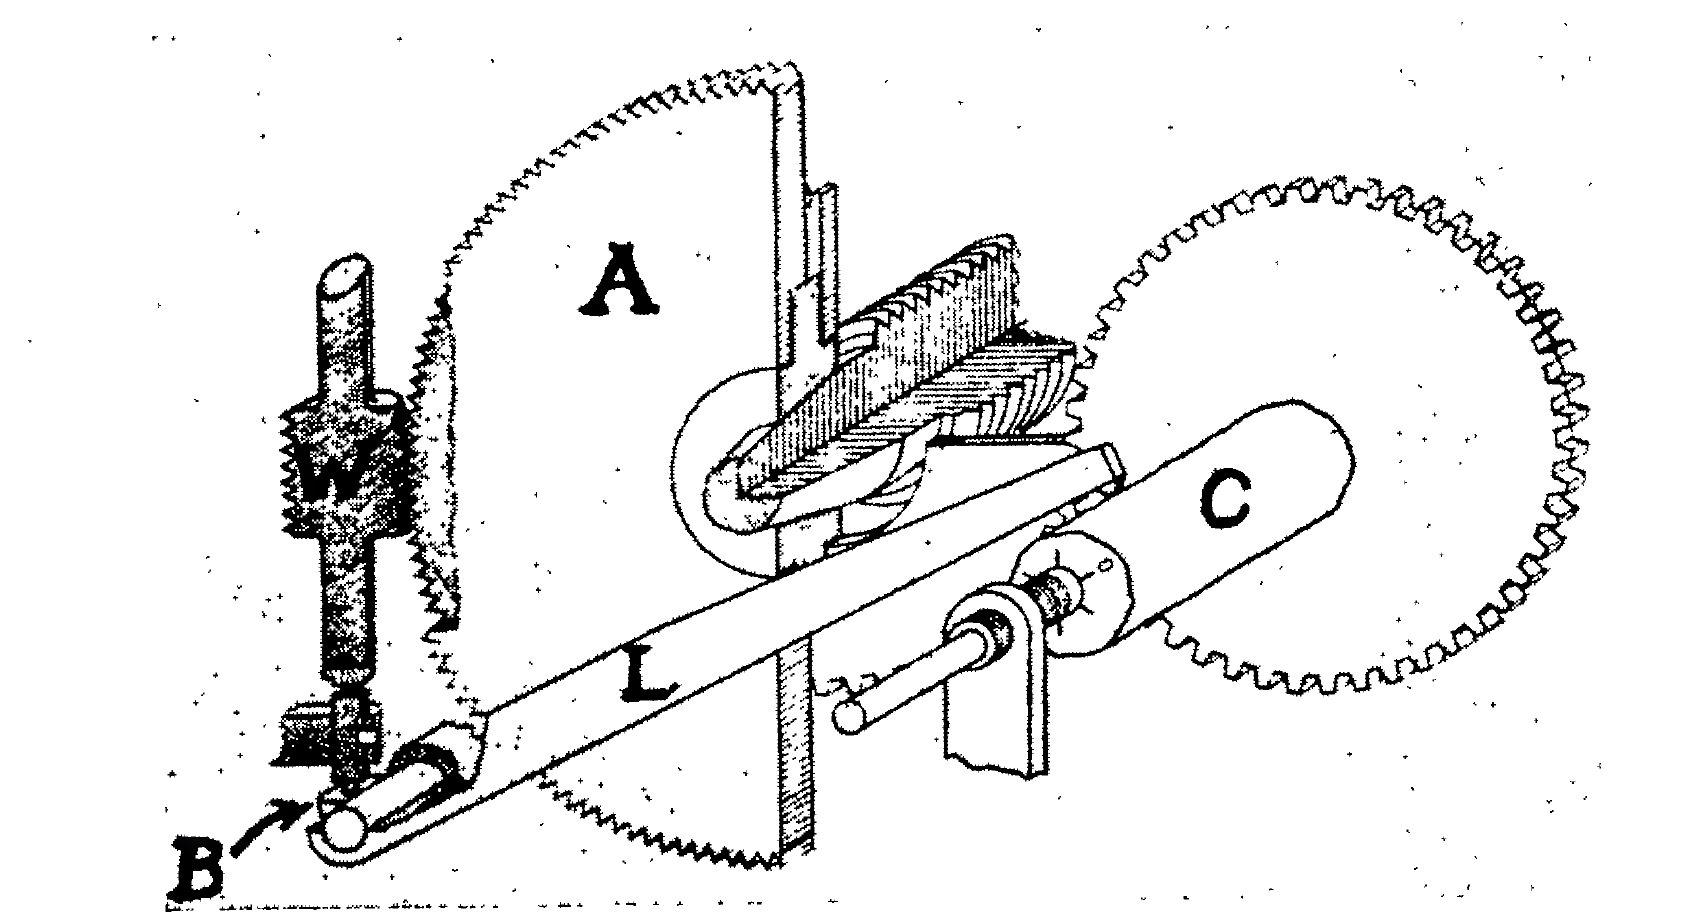
\includegraphics[width=0.8\textwidth]{engine.png}
\end{center}
\caption{Управляющий механизм делительной машины}
\label{fig:engine}
\end{figure}

Для решётки 600 штр/мм для зелёной спектральной линии ртути в 3 порядке наблюдается линия как на рис.~\ref{fig:mercury}(a). При добавлении ошибки $d_1 \sin{\theta}$ с таким периодом, что $d_1 / d_0 = 0,1274$, результат будет как на рис.~\ref{fig:mercury}(b). Главная линия исчезает и по бокам наблюдаются <<духи>> 1-го и 2-го порядков. Если увеличить $d_1 / d_0$ до $0,203$ таким образом, что $2 \pi N \frac{d_1}{d_0} = 3,832$, результат будет как на рис.~\ref{fig:mercury}(c). Первый <<призрак>> исчезает, а основная линия и второй <<призрак>> имеют одинаковую интенсивность, что согласуется с теорией.

\begin{figure}[h!]
\begin{center}
    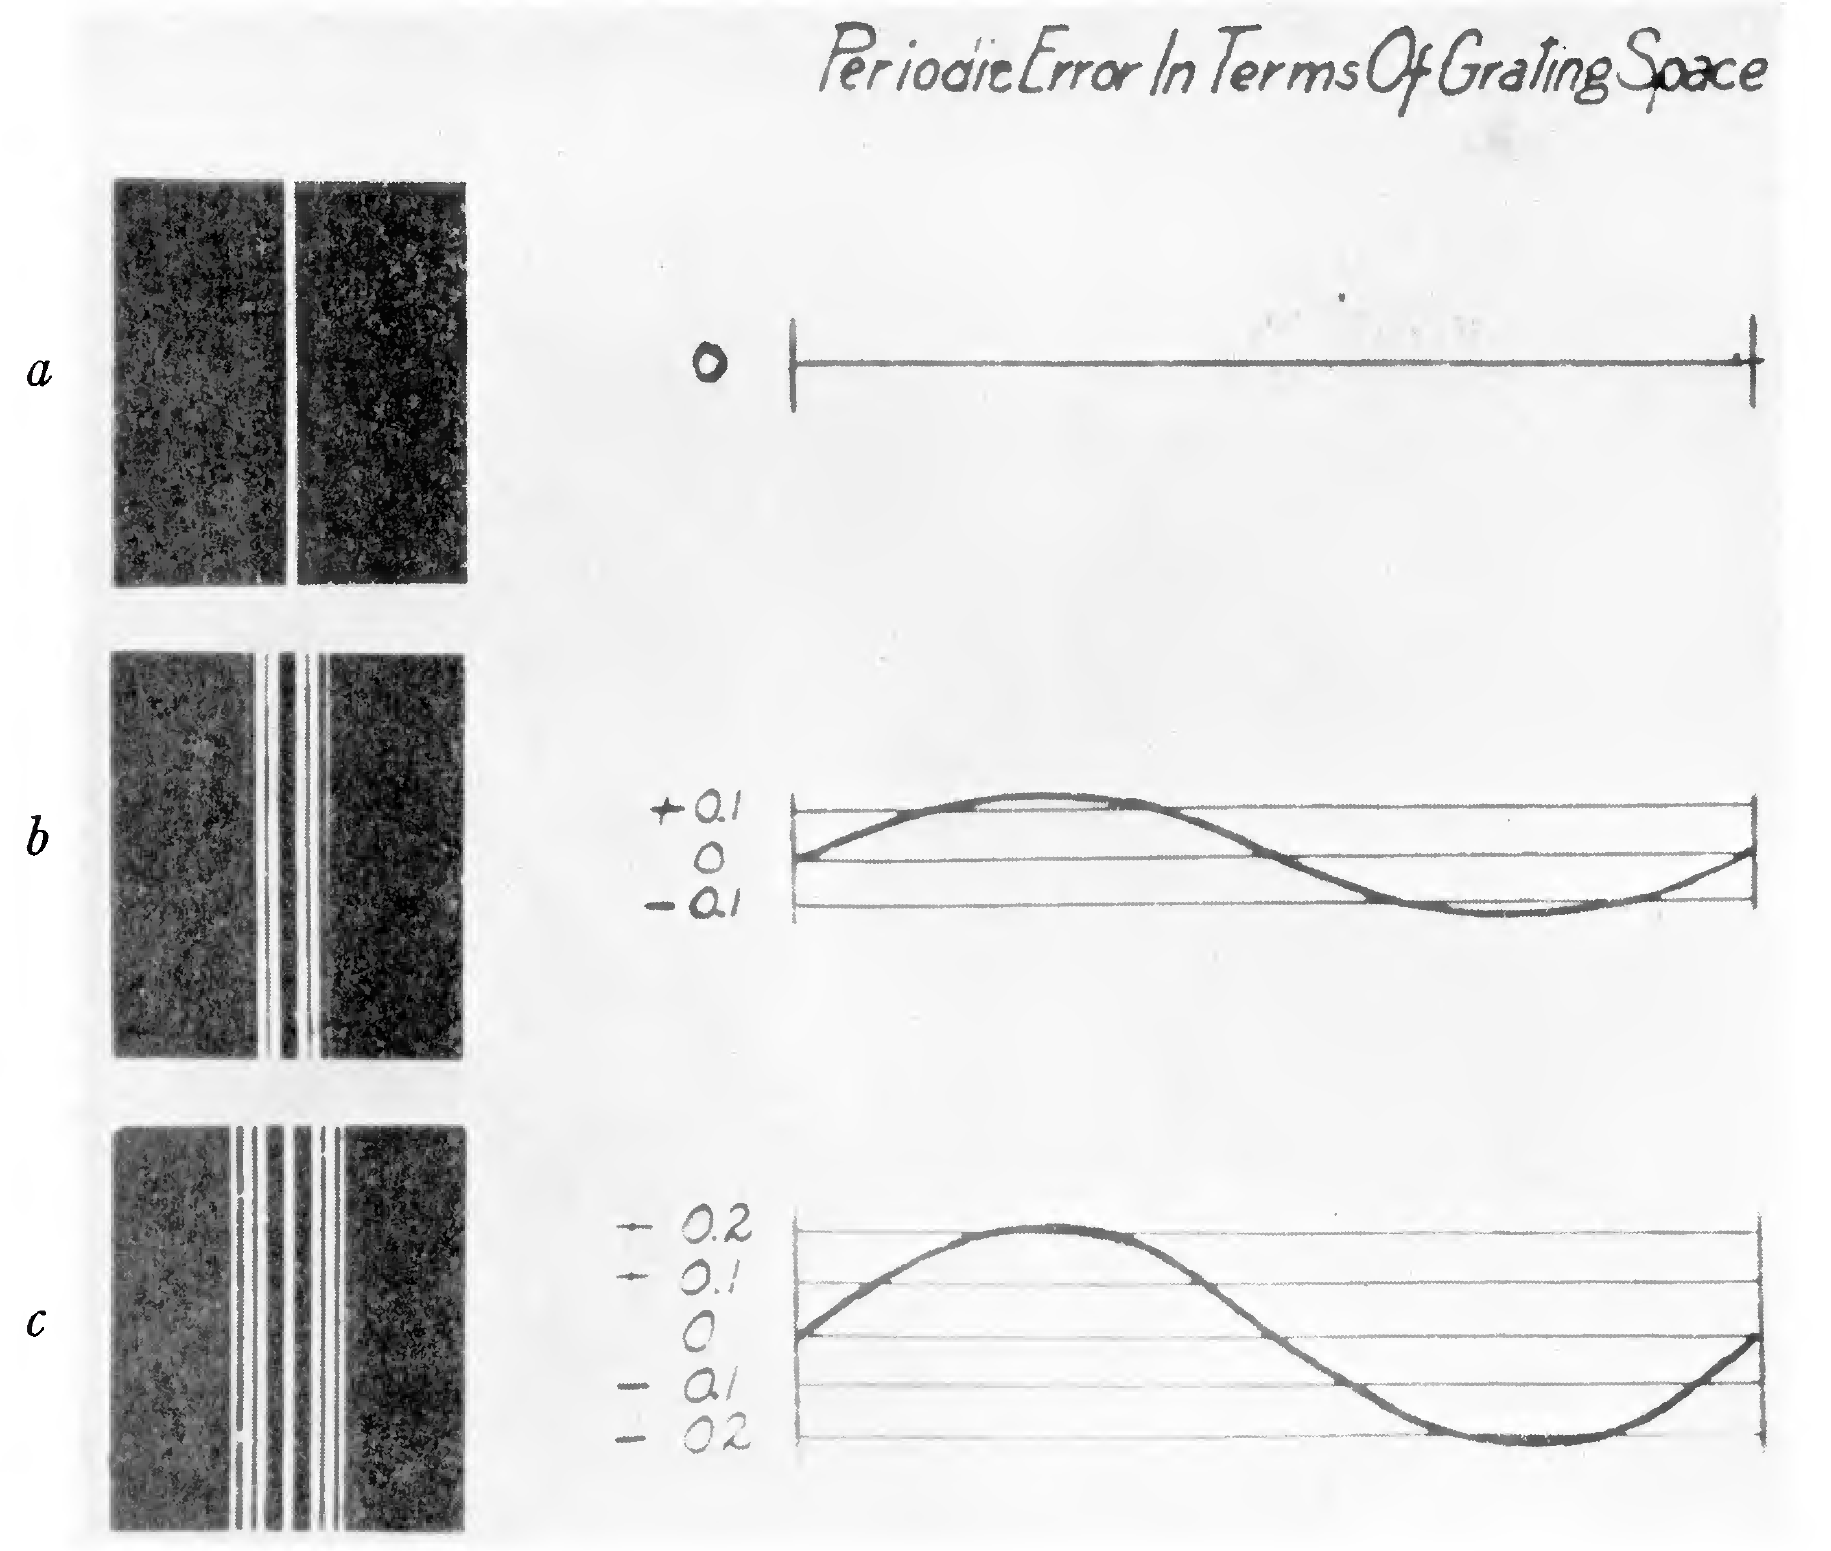
\includegraphics[width=0.8\textwidth]{mercury.png}
\end{center}
\caption{<<Духи>> Роуланда для зелёной линии ртути в 3-м порядке дифракции}
\label{fig:mercury}
\end{figure}

Для демонстрации зависимости от порядка дифракционного максимума, возьмём спектр 2-го, 3-го и 4-го порядков. Соответствующие значения $u = 2 \pi N \frac{d_1}{d_0}$: $1,604$, $2,405$ и $3,208$. Результаты изображены на рис.~\ref{fig:orders}(a), (b), (c).

\begin{figure}[h!]
\begin{center}
    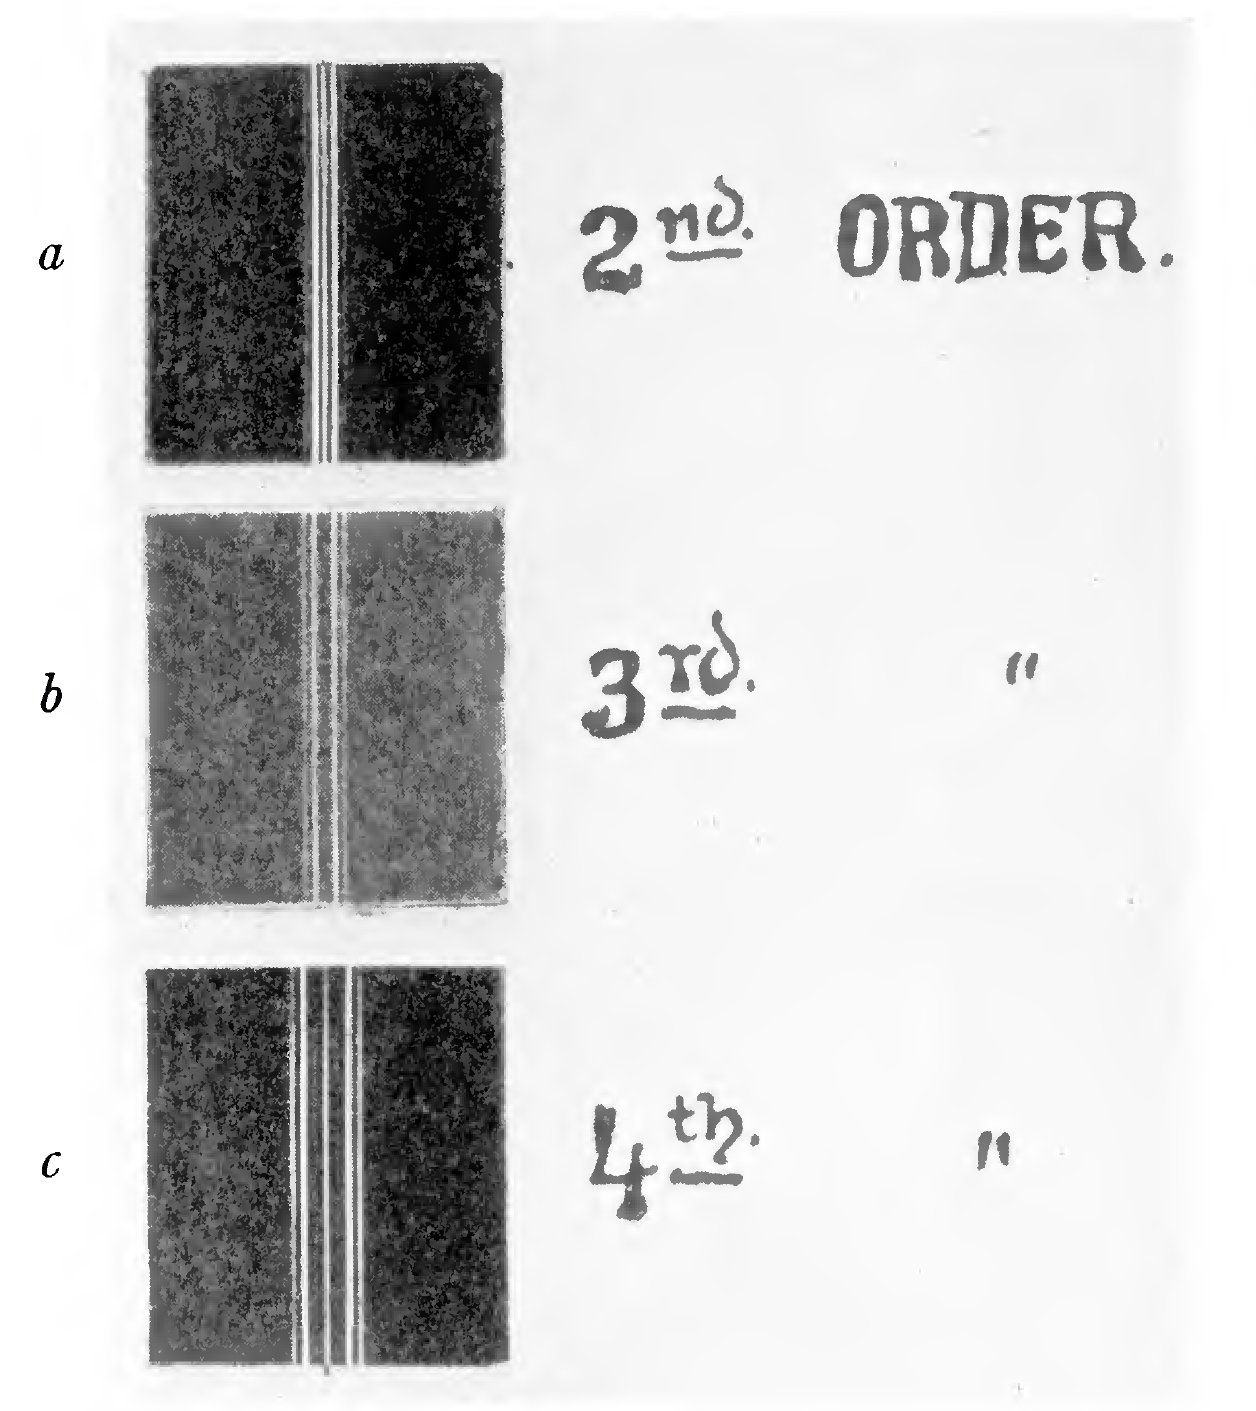
\includegraphics[width=0.5\textwidth]{orders.png}
\end{center}
\caption{<<Духи>> Роуланда в зависимости от порядка спектра}
\label{fig:orders}
\end{figure}

Однако, призрак любого порядка --- 3-го, 5-го, 8-го и т. д. --- можно получить добавлением ошибки $d_1 \sin{3\theta}$, или $d_1 \sin{5\theta}$, или $d_1 \sin{8\theta}$, и т. д. Ошибки $d_1 \sin{8\theta}$ и $d_1 \sin{7\frac{1}{2}\theta}$ приводят к появлению <<призраков>> 8-го порядка в первом случае и на позиции $7\frac{1}{2}$, на середине между 7-м и 8-м порядками, как показано на рис.~\ref{fig:periods}(a) и (b). На рис.~\ref{fig:periods}(c) показаны <<духи>> 7-го и 8-го порядков одинаковой интенсивности.

\begin{figure}[h!]
\begin{center}
    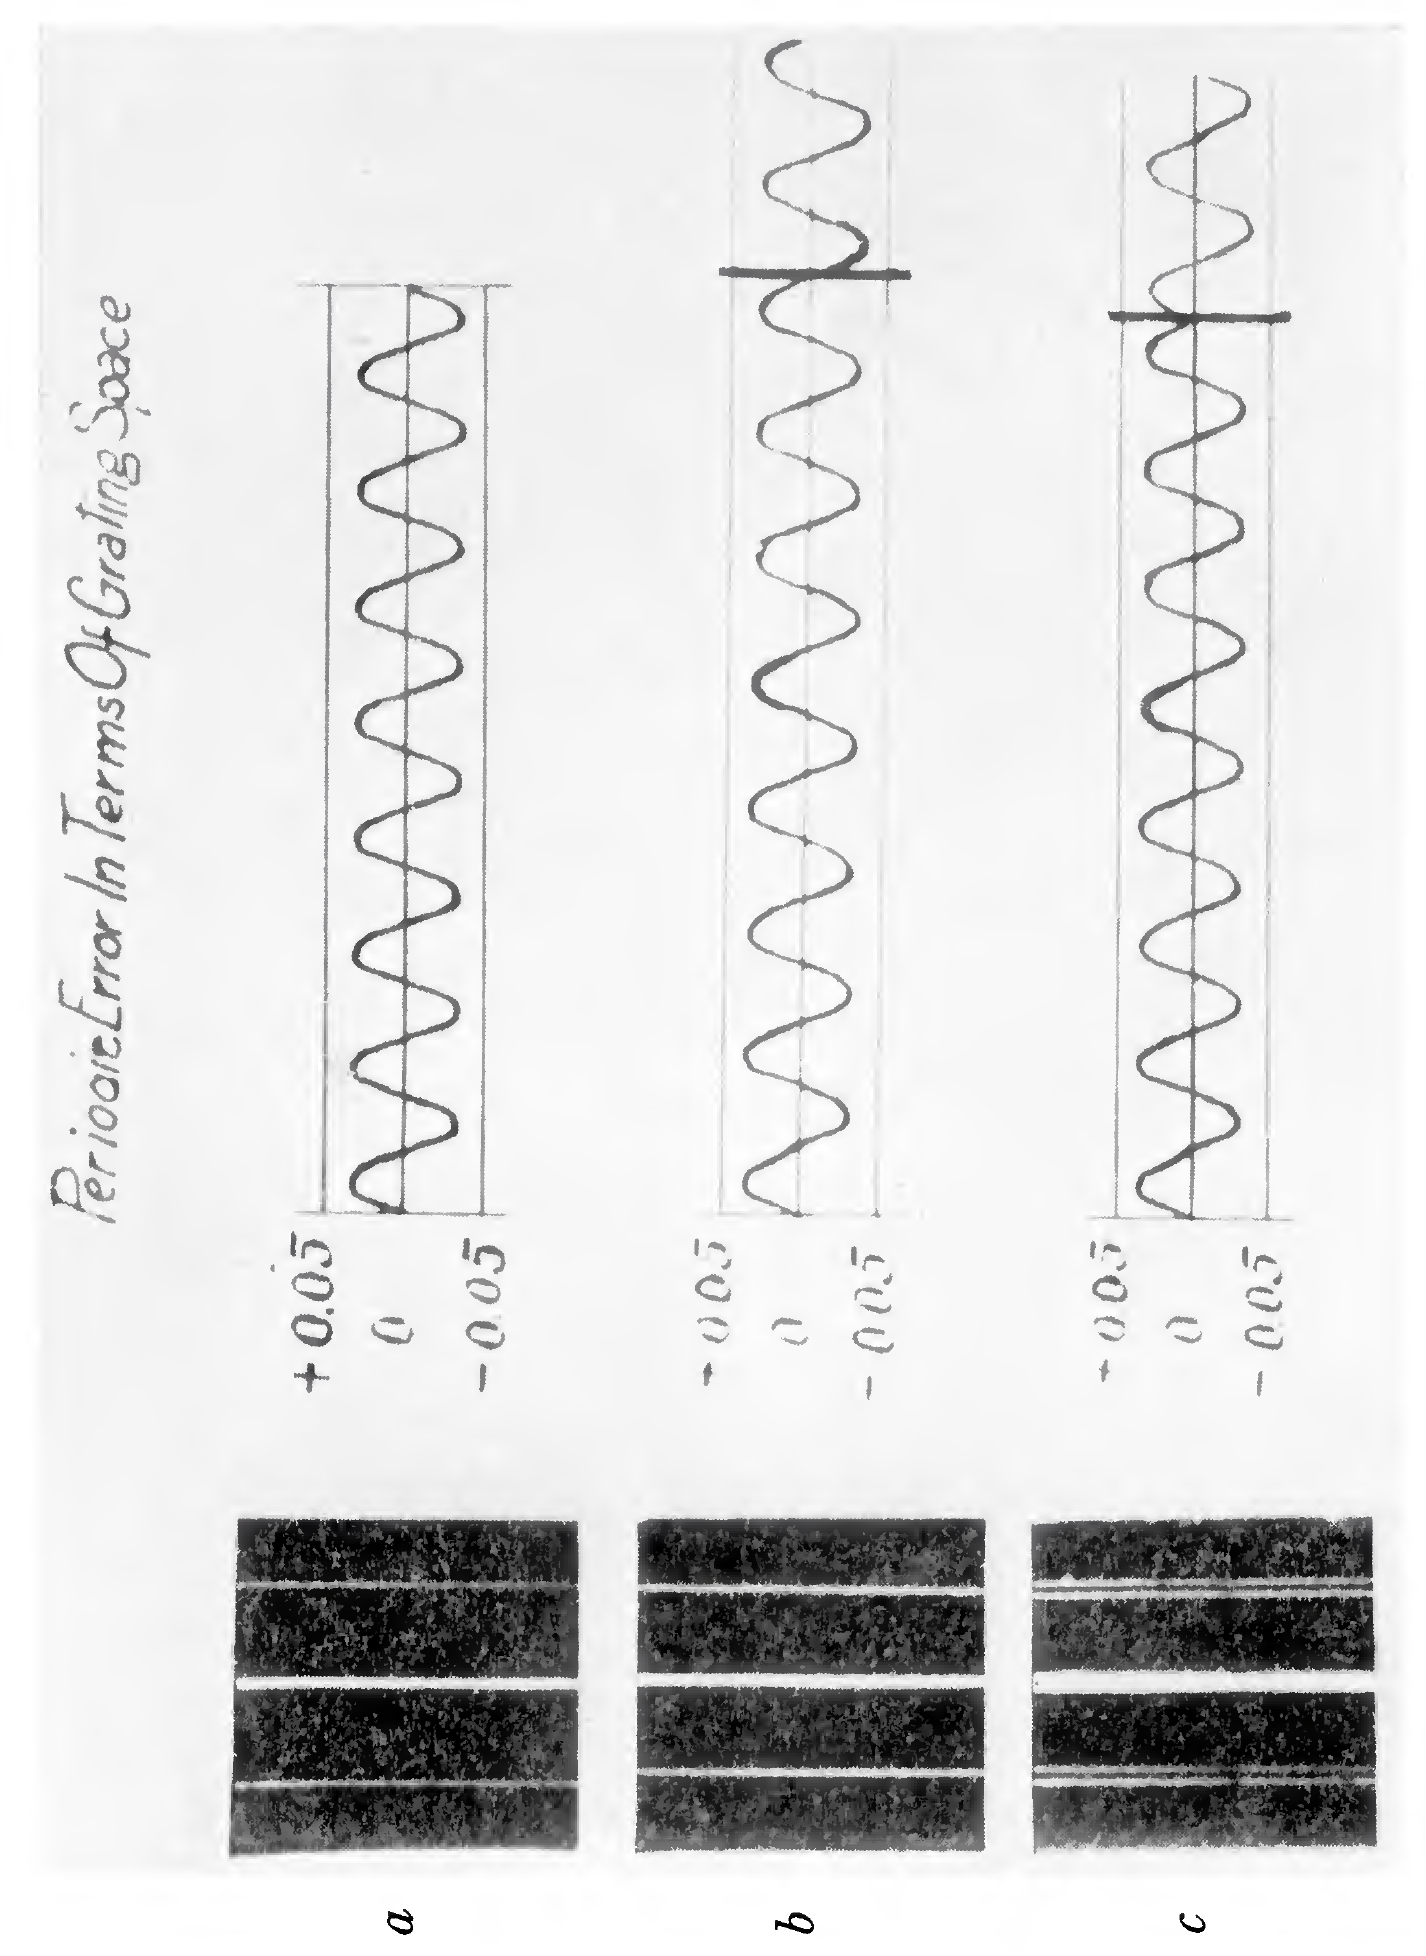
\includegraphics[width=0.51\textwidth]{periods.png}
\end{center}
\caption{<<Духи>> Роуланда высоких порядков}
\label{fig:periods}
\end{figure}

При добавлении ошибки $d_1 \sin{8\frac{1}{3}\theta}$, которая после каждого оборота начиналась бы в одной фазе, <<духи>> появляются в 8-м и 9-м порядках, но <<дух>> 8-го порядка имеет в 4 раза б\'{о}льшую интенсивность, как показано на рис.~\ref{fig:sum_periods}(a). Когда были добавлены ошибки $d_1 \sin{7\theta}$ и $d_1 \sin{8\theta}$ одновременно, одинаковые <<призраки>> появлялись на 7 и 8 позициях. Аналогичные результаты были получены для ошибок $d_1 \sin{5\theta}$ и $d_1 \sin{8\theta}$, как показано на рис.~\ref{fig:sum_periods}(b) и (с).

\newpage

\begin{figure}[h!]
\begin{center}
    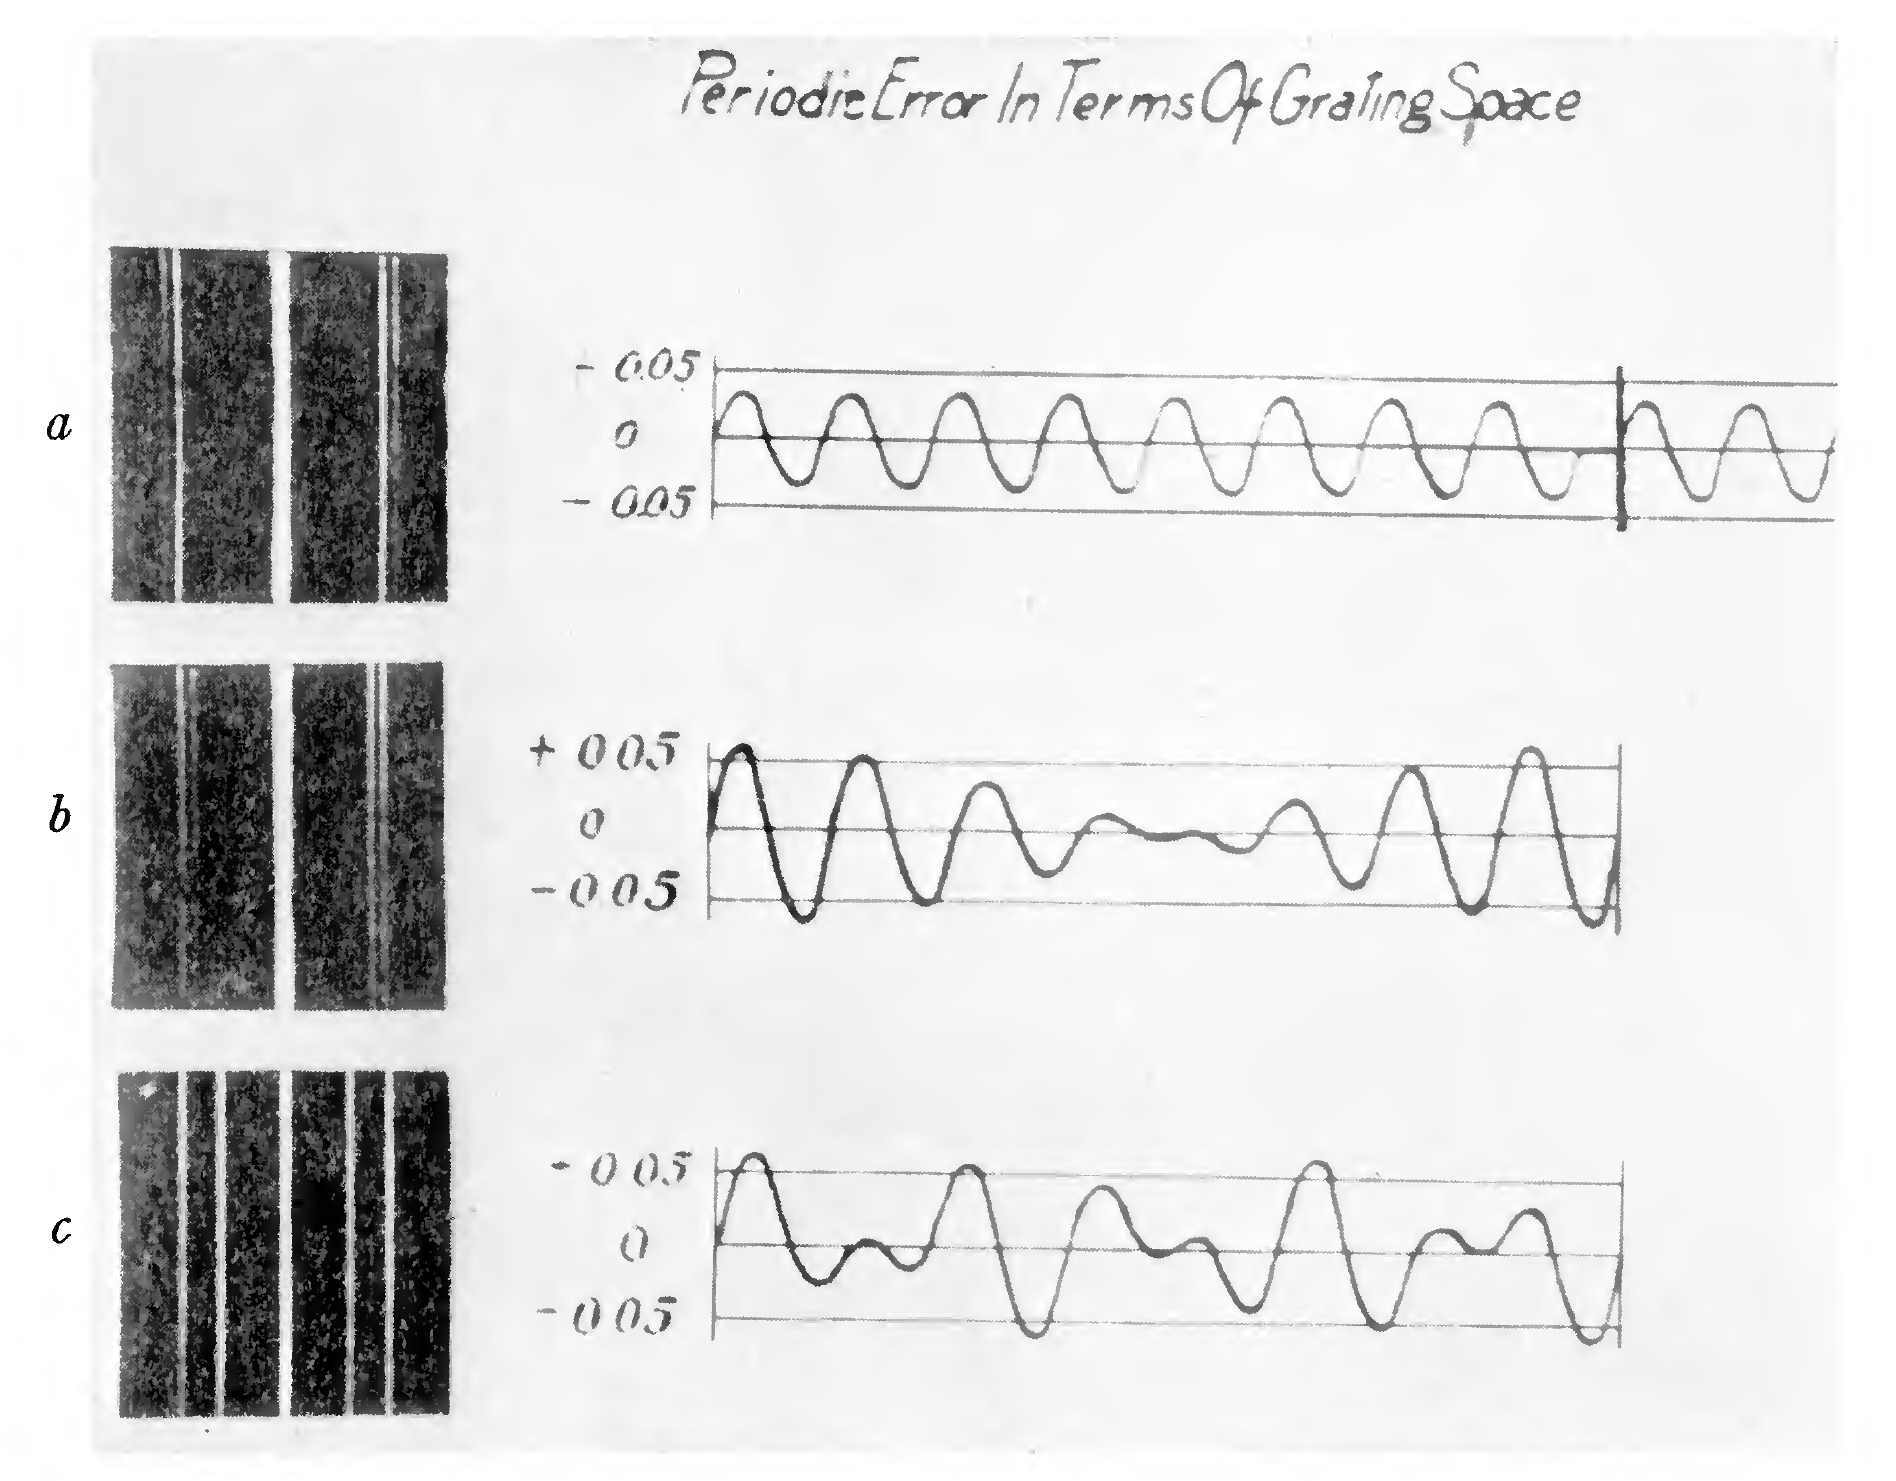
\includegraphics[width=0.8\textwidth]{sum_periods.png}
\end{center}
\caption{<<Духи>> Роуланда при сложении ошибок}
\label{fig:sum_periods}
\end{figure}

\begin{thebibliography}{99}
\bibitem{A-P Journal}
The Astrophysical Journal. V. 85, N. 2. March, 1937. Henry G. Gale. Rowland Ghosts.
\bibitem{Rowland}
Physical Papers of Henry A. Rowland. с. 525.
\end{thebibliography}

%\newpage
%
%\begin{picture}(\textwidth ,5)
%\linethickness{5mm}
%\put(0,1){\line(1,0){\textwidth}}
%\end{picture}
%
%\vspace{1 cm}
%
%\begin{tikzpicture}
%\draw [line width=3mm, black] (0, 0) -- ++(4, 0) -- ++(0, -6) -- ++(-4, 0) -- ++(0, 6) -- ++(4, 0);
%\foreach \i in {0,1,...,100}{
%    \draw [line width=0.04mm, black] (1, -1-\i*0.04) -- (3,-1-\i*0.04);
%}
%\end{tikzpicture}


\end{document}
